\documentclass[a4paper,11pt]{article}
\usepackage[utf8]{inputenc}
\usepackage[T1]{fontenc}
\usepackage[french]{babel}
\usepackage{graphicx}
\usepackage{lipsum}
\usepackage[a4paper]{geometry}
\usepackage{wallpaper}
\usepackage{libertine}
\usepackage{csquotes}
\usepackage{fancyhdr}
\usepackage{vmargin}
\usepackage{hyperref}
\usepackage[colorinlistoftodos]{todonotes}
\usepackage{titlesec}
\usepackage{array}



\makeatletter
\def\clap#1{\hbox to 0pt{\hss #1\hss}}%
\def\ligne#1{%
\hbox to \hsize{%
\vbox{\centering #1}}}%
\def\haut#1#2#3{%
\hbox to \hsize{%
\rlap{\vtop{\raggedright #1}}%
\hss
\clap{\vtop{\centering #2}}%
\hss
\llap{\vtop{\raggedleft #3}}}}%
\def\bas#1#2#3{%
\hbox to \hsize{%
\rlap{\vbox{\raggedright #1}}%
\hss
\clap{\vbox{\centering #2}}%
\hss
\llap{\vbox{\raggedleft #3}}}}%
\def\maketitle{%
\thispagestyle{empty}\vbox to \vsize{%
\haut{}{\@blurb}{}
\vfill
\vspace{1cm}
\begin{flushleft}
\usefont{OT1}{ptm}{m}{n}
\huge \@title
\end{flushleft}
\par
\hrule height 4pt
\par
\begin{flushright}
\usefont{OT1}{phv}{m}{n}
\Large \@author
\par
\end{flushright}
\vspace{1cm}
\vfill
\vfill
\bas{}{\@location, le \@date}{}
}%
\cleardoublepage
}
\def\date#1{\def\@date{#1}}
\def\author#1{\def\@author{#1}}
\def\title#1{\def\@title{#1}}
\def\location#1{\def\@location{#1}}
\def\blurb#1{\def\@blurb{#1}}
\Large{\date{\today}}
\author{}
\title{}
\location{Rennes}\blurb{}
\makeatother
\title{\LARGE{Projet Modélisation et Programmation Orientée Objet}}
\author{Frank \textsc{Chassing} et Amandine \textsc{Fouillet}}
\location{Rennes}
\blurb{%
\large{INSA de Rennes\\
\textbf{Rapport de conception}}
}%


\begin{document}
\maketitle
\tableofcontents
\newpage
\section*{Introduction}


\section{Diagrammes de cas d'utilisation}
\begin{figure}[h!]
\fbox{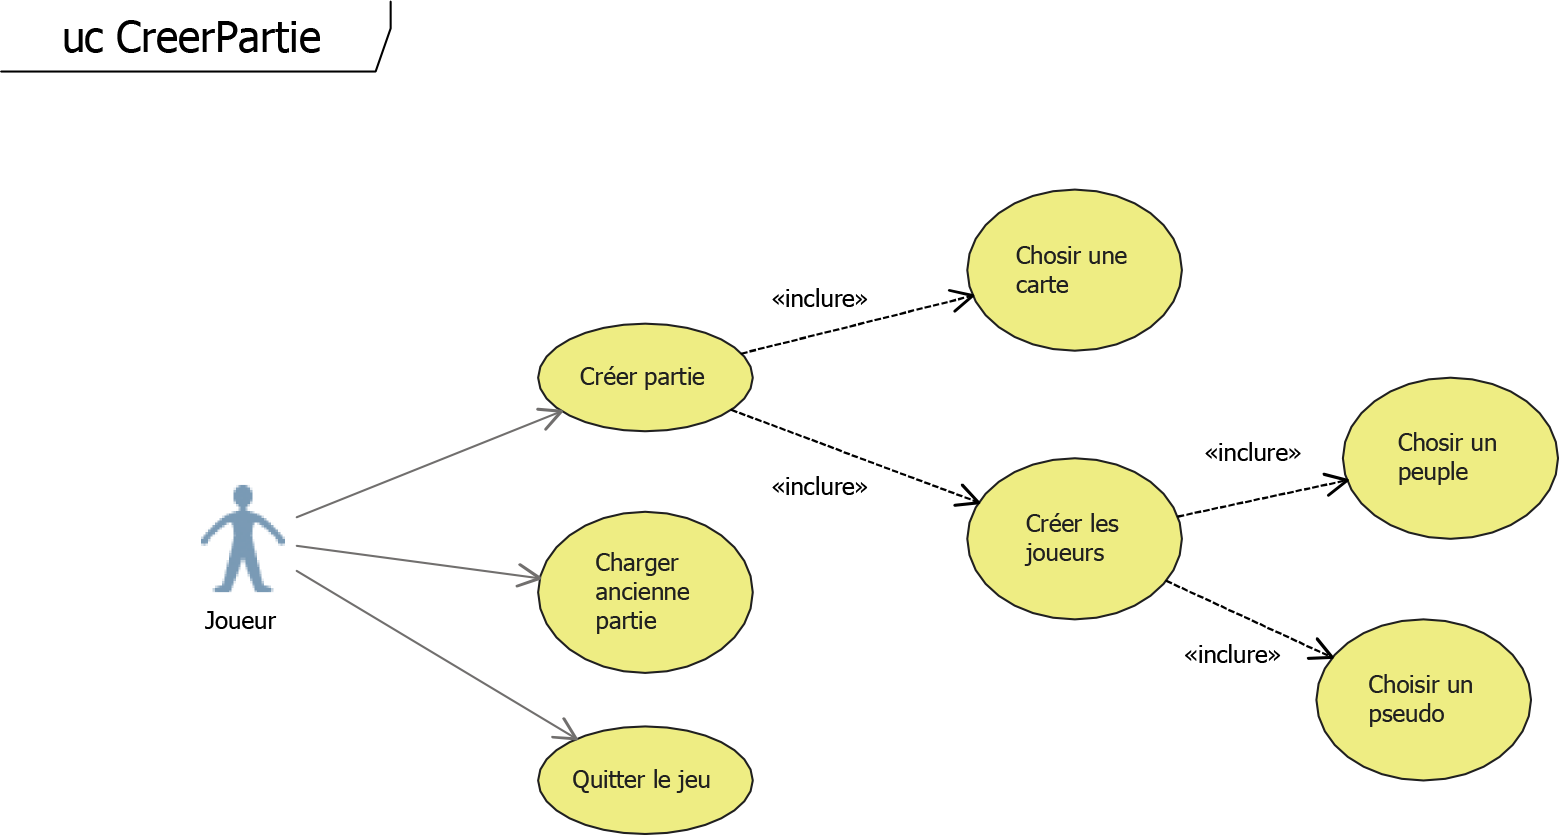
\includegraphics{ucCreerPartie.png}}
\caption{Cas d'utilisation - Créer une Partie}
\end{figure}
~\\
\begin{figure}[h!]
\fbox{\includegraphics{ucTourDeJeu.png}}
\caption{Cas d'utilisation - Créer une Partie}
\end{figure}



\section{Diagrammes d'activités}
\begin{figure}[h]
\fbox{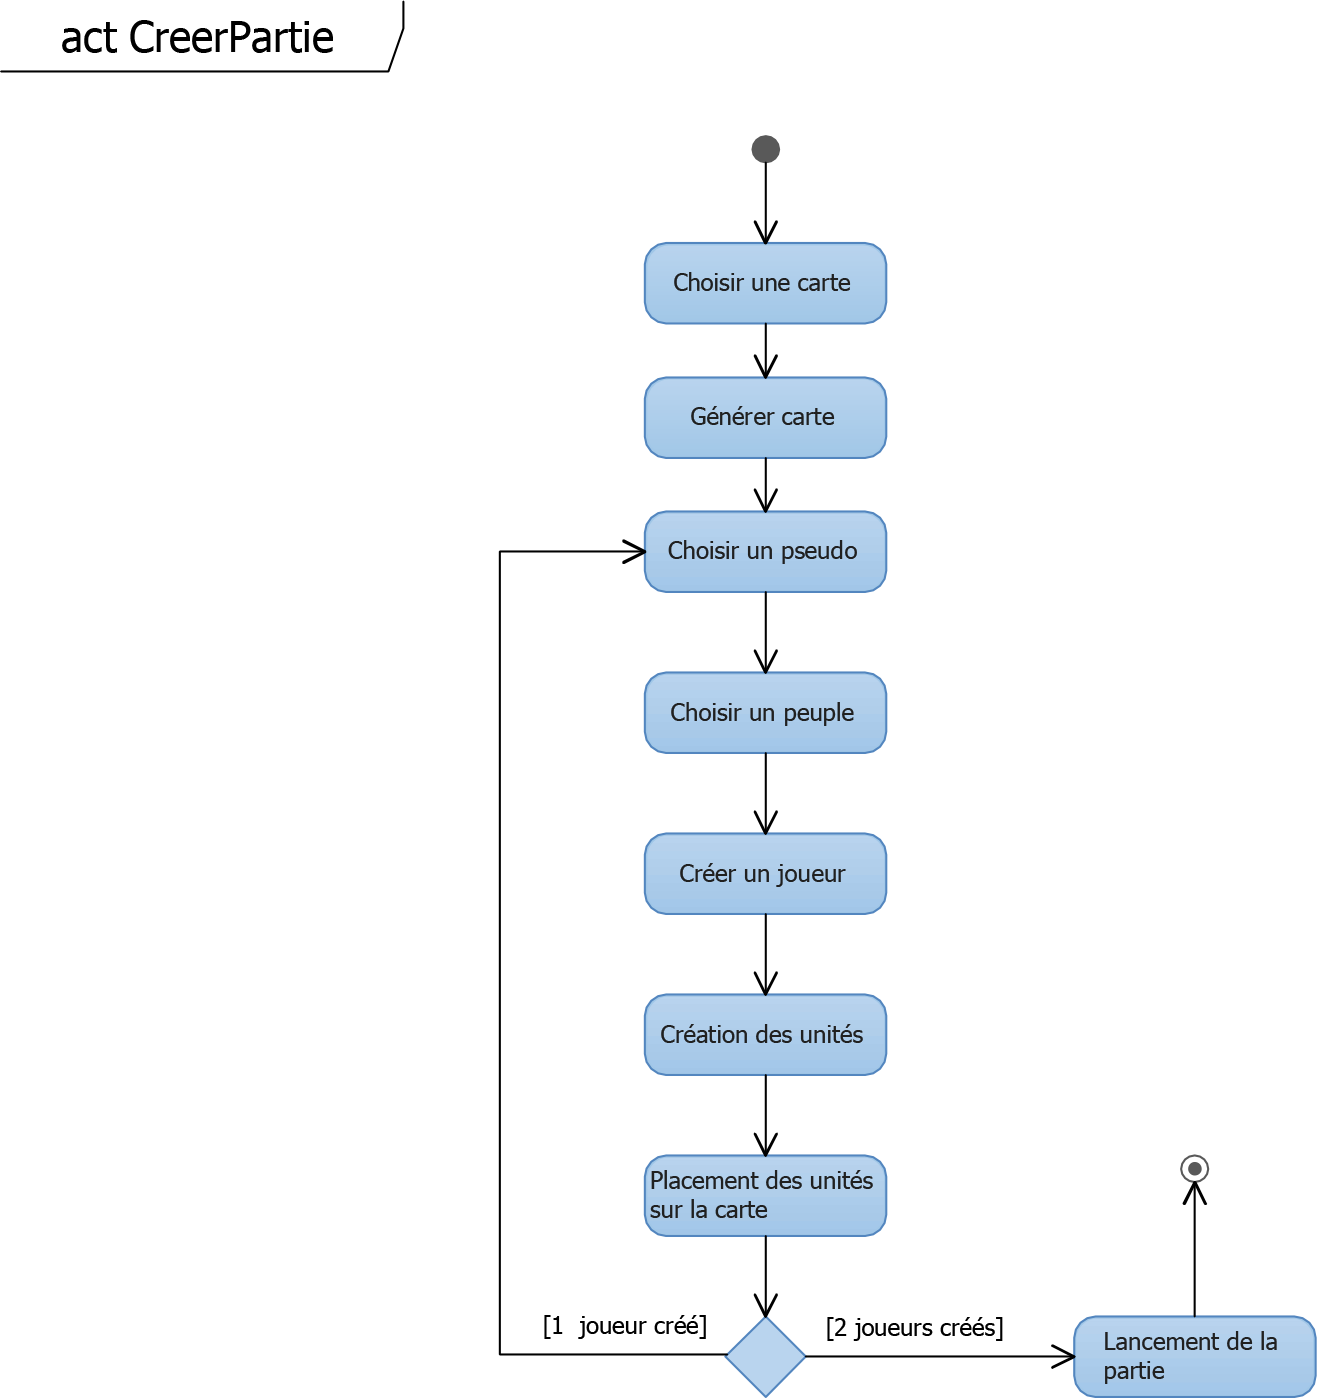
\includegraphics{actCreerPartie.png}}
\caption{Cas d'utilisation - Créer une Partie}
\end{figure}
~\\
\begin{figure}[h!]
\fbox{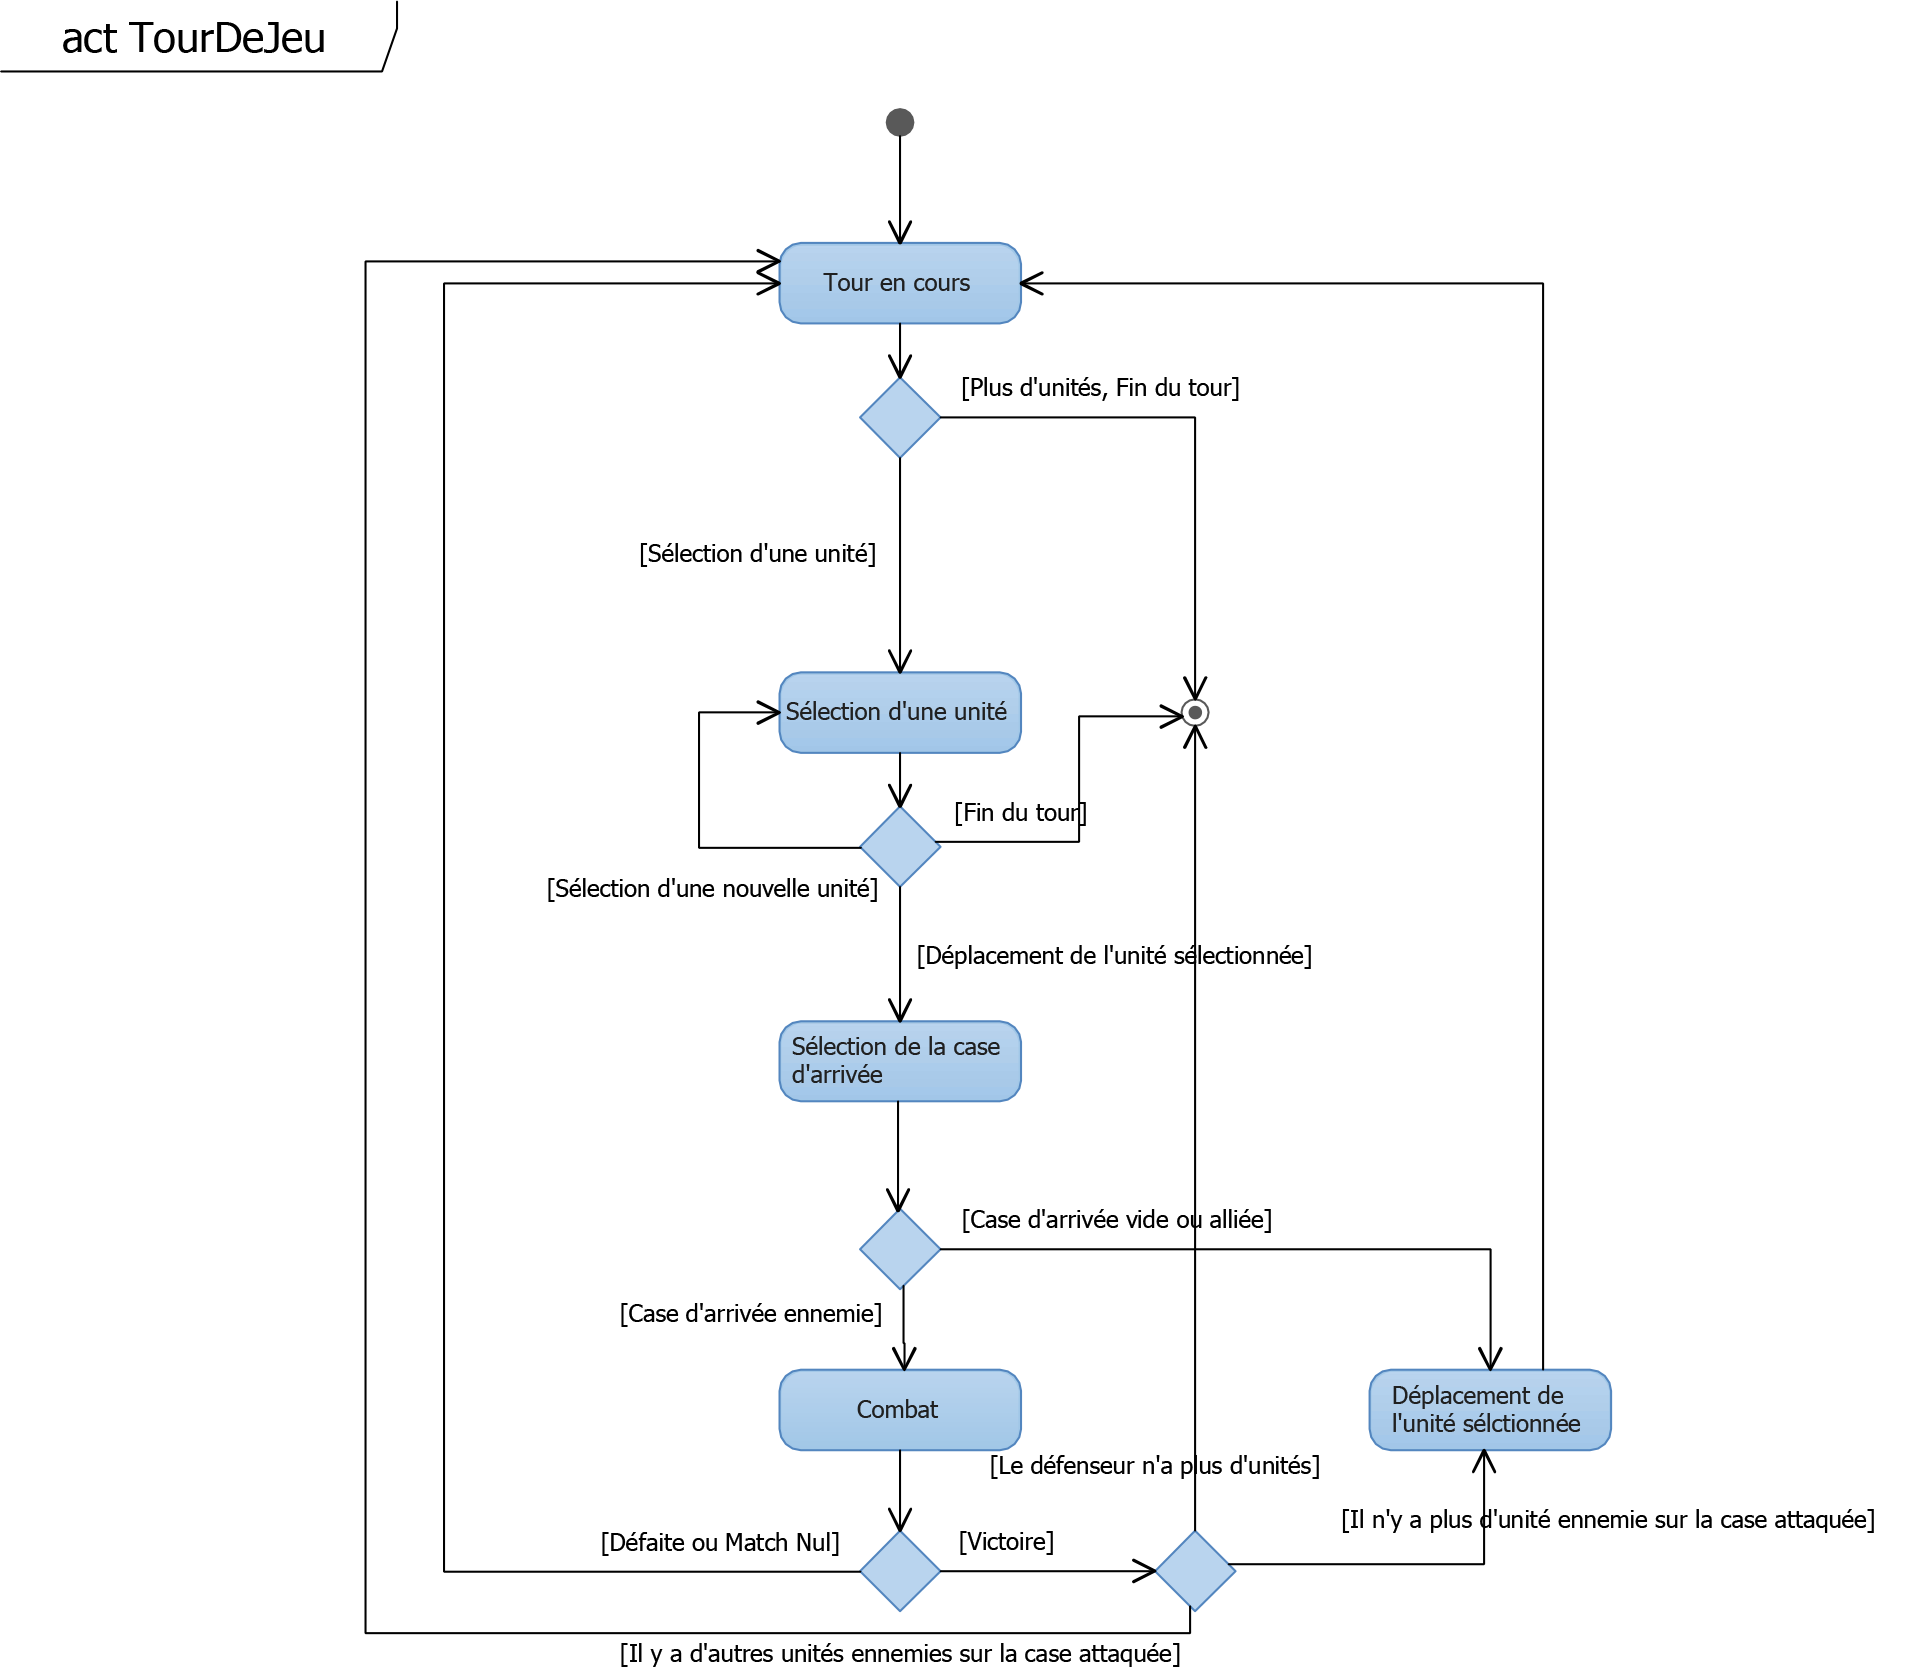
\includegraphics{actTourDeJeu.png}}
\caption{Cas d'utilisation - Créer une Partie}
\end{figure}
~\\
\begin{figure}[h!]
\fbox{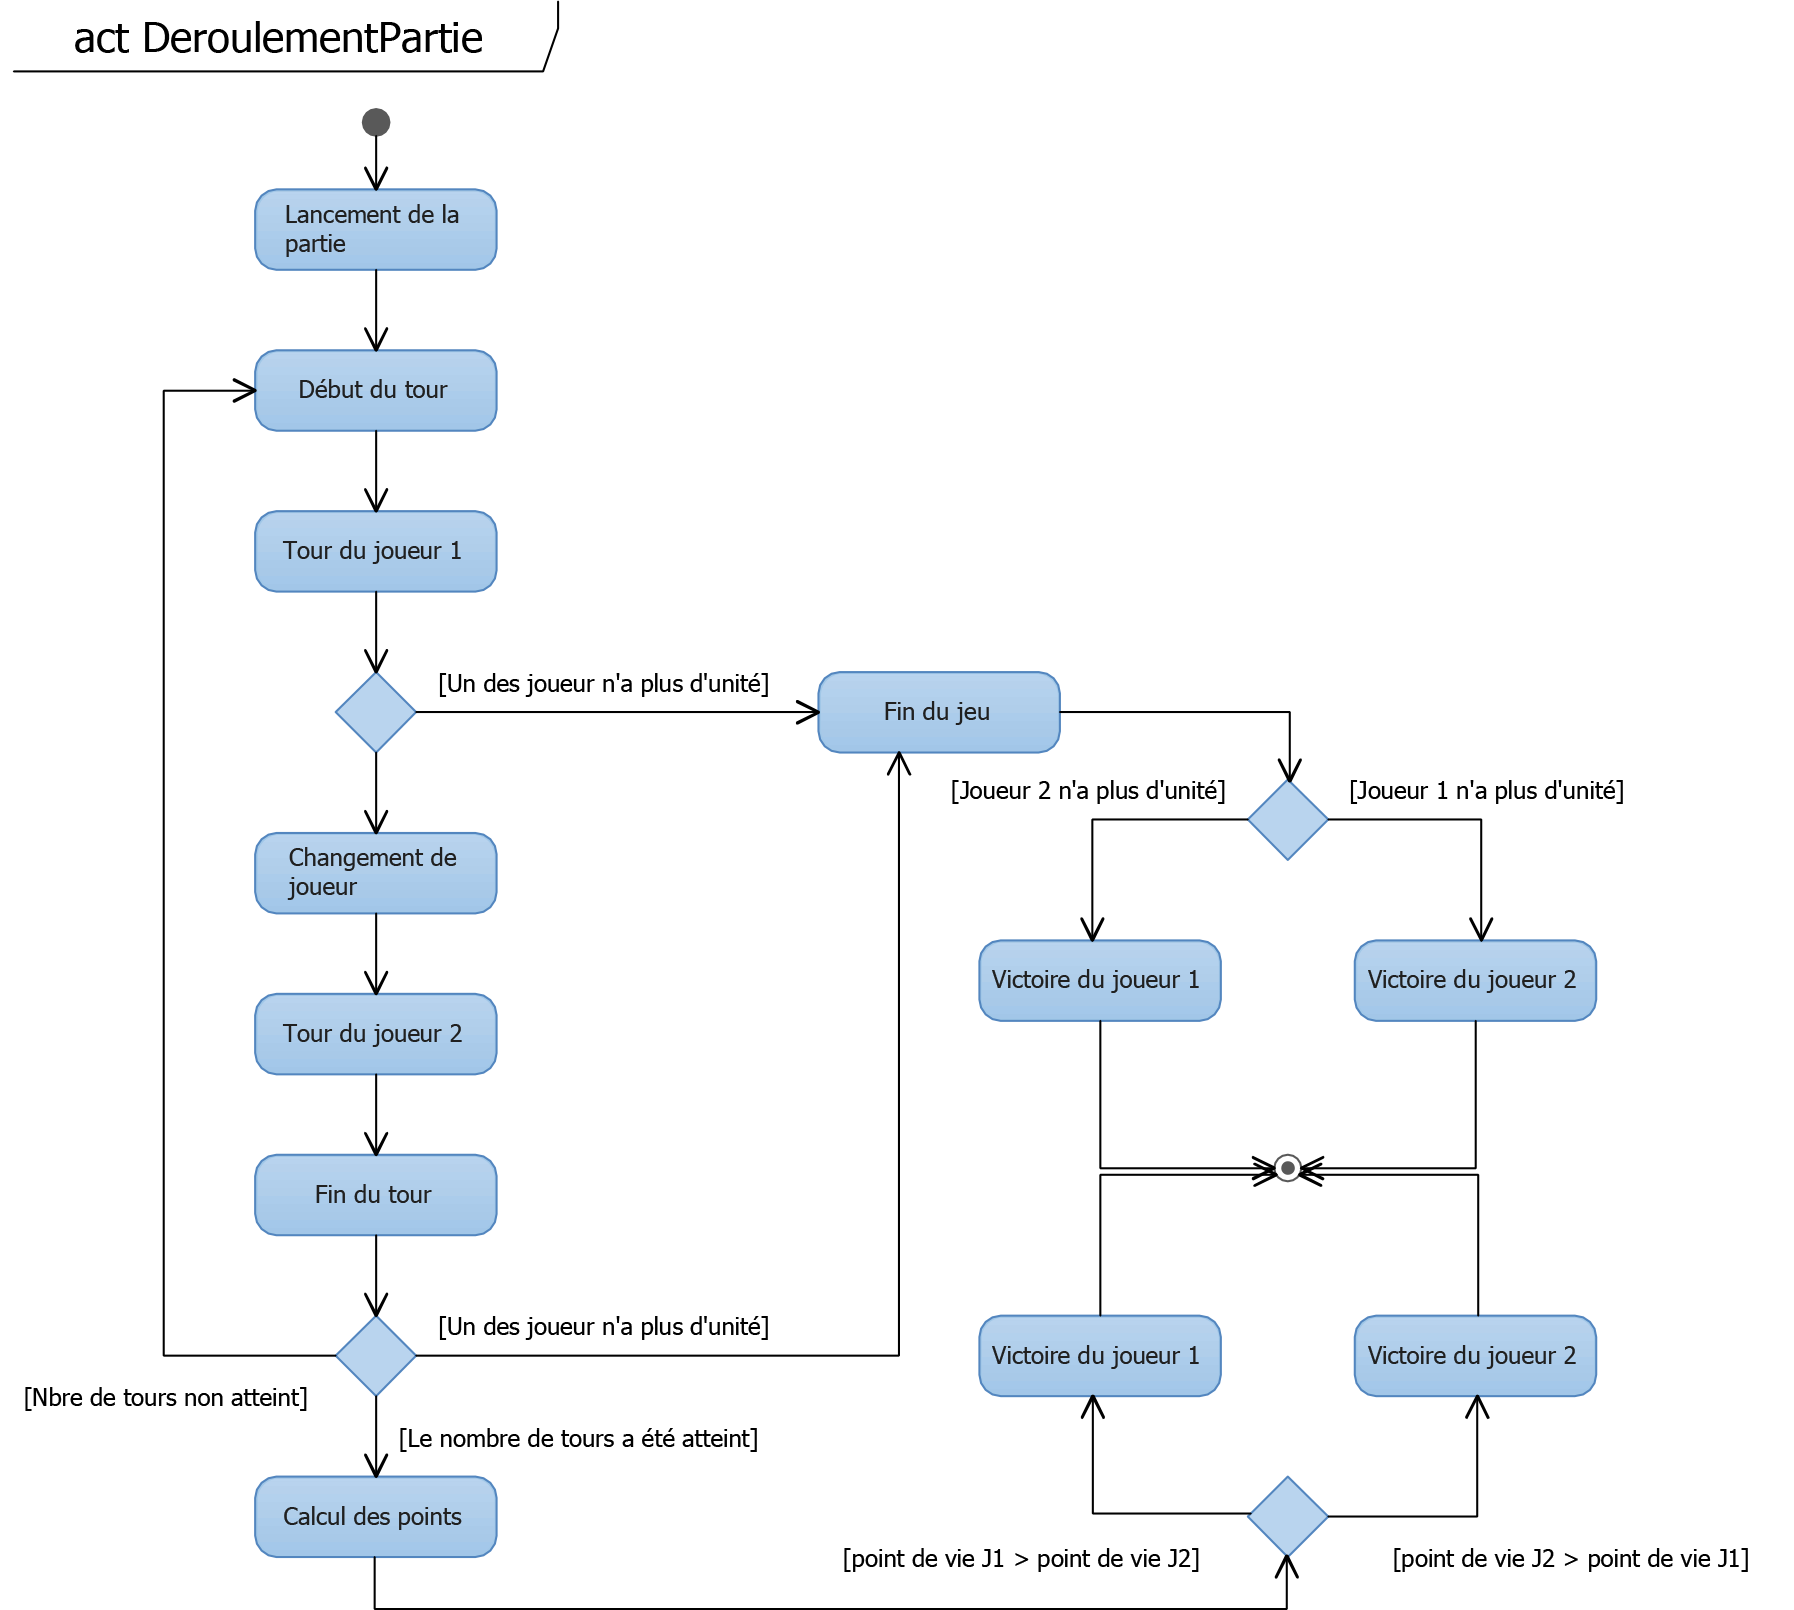
\includegraphics{actDeroulementPartie.png}}
\caption{Cas d'utilisation - Créer une Partie}
\end{figure}
~\\
\begin{figure}[h!]
\fbox{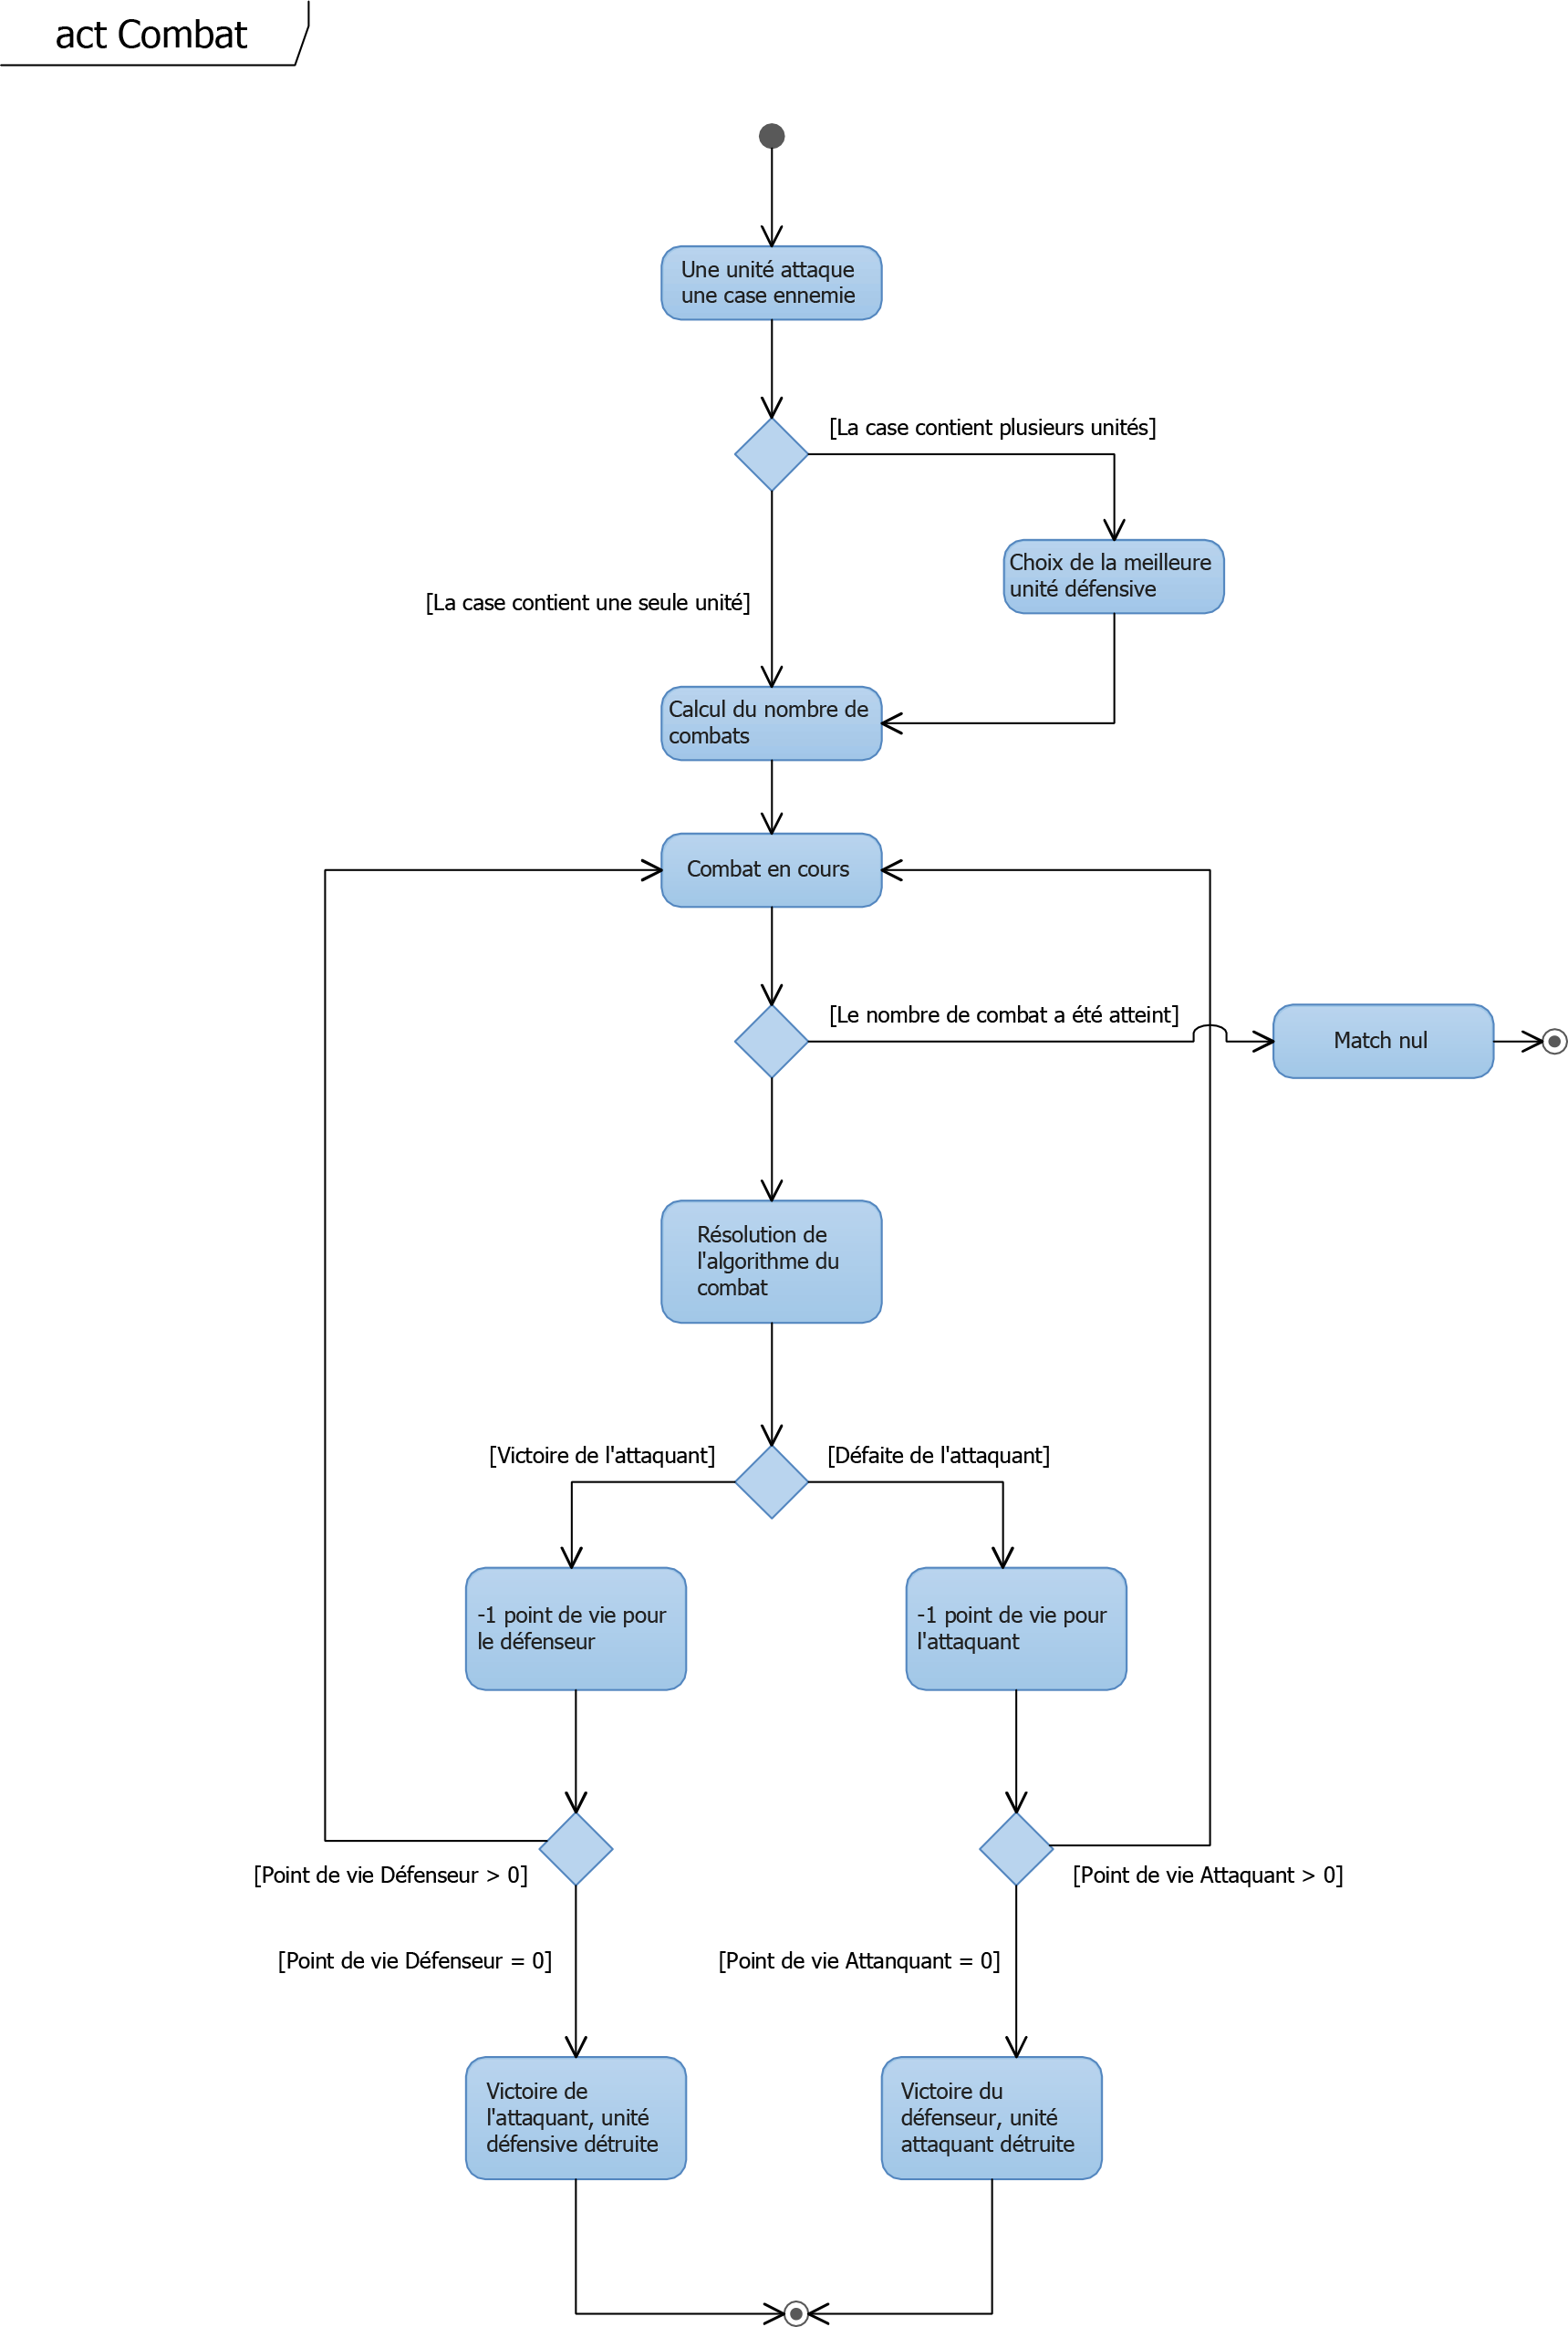
\includegraphics{actCombat.png}}
\caption{Cas d'utilisation - Créer une Partie}
\end{figure}
~\\

\section{Diagramme d'états-transitions}
AHAHAH

\section{Diagramme de séquence}
\begin{figure}[h!]
\fbox{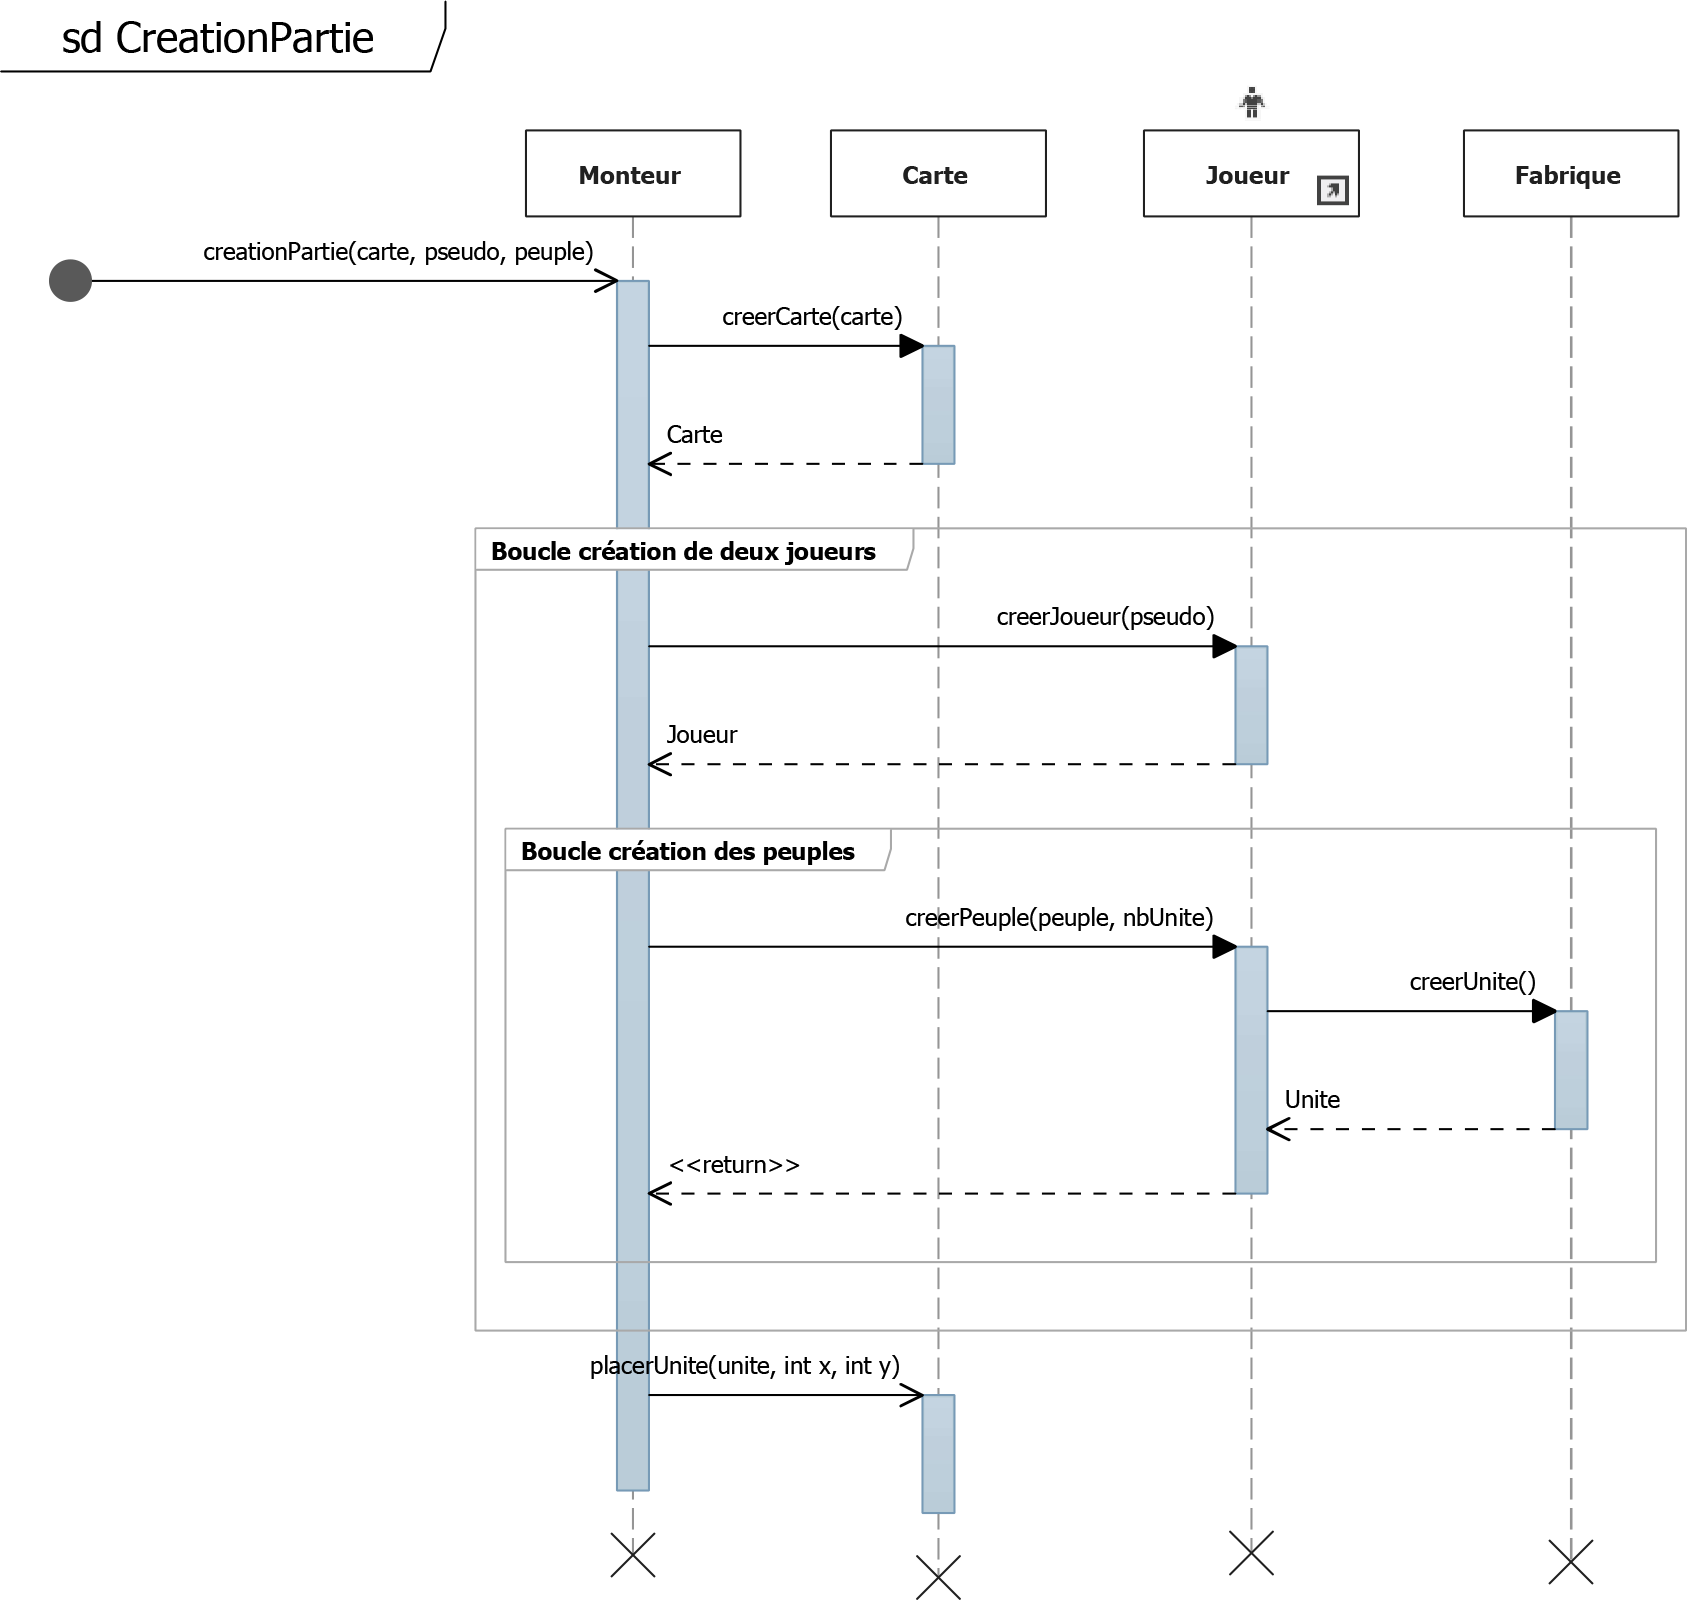
\includegraphics{sqCreerPartie.png}}
\caption{Cas d'utilisation - Créer une Partie}
\end{figure}
~\\

\section{Diagramme de classe}
A récupérer

\section*{Conclusion}
\end{document}